\section{Analysis}
\subsection{Overview of Claims \& Introduction to Analysis}

We will show that a student used different strategies to decide how to look at code in two different problems and that each strategy appeared to help him understand unfamiliar constructs, which then allowed him to solve the problem.
For the evaluation problem, where the code passed a function as an argument, the student evaluated the code in the order it would have been executed.
For the debugging problem, where there was a bug in the Connect 4 gameplay code, the student started looking at the code at the top of the paper and continued down until reaching a likely candidate for the location of the bug.
We include two partial transcripts from a debugging and an evaluation problem to support these claims. 
In the presented transcript, the symbol [...] indicates where we removed portions of the transcript in order to focus on the parts of the transcripts that are integral to our analysis. 
The full transcript of each question is provided in Appendix \ref{sec-full-transcripts}. 
This student had taken a couple of computer science classes at Harvey Mudd College, including Principles and Practices of Computer Science, Data Structures and Program Development, and had tutored extensively for the Data Structures and Program Development class.

%\newpage
\subsection{Q1: Evaluation}

The analysis begins from when the student is handed the first problem.
The program starts with a call to main on line 18, and main is defined on line 12.

\begin{lstlisting}[language=python]
12		def main():
13			print(func3([1,2,3,4]))
...
18		main()
\end{lstlisting}

The student began by identifying the call to main, as shown in the section of transcript below:

\begin{tabular}{lp{13cm}}
T1&Alright so, its got a main, so thats gonna start. [...]\\
\end{tabular}

The student started at the main function. It is the very first thing he identified even though the function is in the middle of the page, and the call to main is not until the end of the page.
He appeared to identify main because he was looking for the start of execution. \\

Omitted from this is transcript is where the student continued in execution order until he reached func2 shown below.
The full transcript is in Appendix \ref{subsec-q1-transcipt}.

\begin{lstlisting}[language=python]
0		def func2(list, num):
1			return func1(list, num, func4)
\end{lstlisting}

The student tried to call func4 instead of passing it to func1.

\begin{tabular}{lp{13cm}}
T2&Function 2 returns function 1 with the same two arguments already passed to it, and function 4, the result of -\\
\end{tabular}

He said ``the result of,'' even though there were no parentheses that would indicate the function was called.
The student appeared to be trying to call func4 before calling func1.

As shown below, the student went to func4 to try to resolve his confusion.

\begin{lstlisting}[language=python]
3		def func4(a, b):
4			return a * b
\end{lstlisting}

He considered ways to call func4 without any arguments, and finished his previous sentence with:

\begin{tabular}{lp{13cm}}
T3&Which doesn't have any implied arguments, thats interesting. Umm, thats odd [pause]\\
\end{tabular}

When he said implied arguments he appears to be referring to default arguments.
In this case he appears to be working off of the hypothesis that if you have default arguments to a function,
  then you can call the function without parentheses (which is incorrect).
However, the student noted that there were no default arguments (he referred to them as implied arguments).
Note that even though the program does not call func4 from func2, because the student believed that func4 is being called, func4 would be executed from the student's perspective. \\

He continued on to func1, even though he still seemed to be confused about how func4 works in func2.

\begin{lstlisting}[language=python]
6		def func1(list, num, f):
7			acc = 0
8			for i in list:
9					acc += f(i, num)
10		return acc
\end{lstlisting}

He noted that the \texttt{f} in func1 is the same as func4 in func2. \\

\begin{tabular}{lp{13cm}}
T4& lets see, so its calling functi-,ooh, it calling function 1.\\
T5&There we go. Uhh, yes, so its calling function with a list a number, the array and 4,\\
T6&and the function 4 as sort of a multiplier.\\
T7&A function to apply. \\
\end{tabular}

In the four lines above, the student was able to figure out that func4 is being passed as an argument.
He noted in T6 that function 4 is being used as a multiplier, and he succinctly described it as ``a function to apply'' in T7.
He appeared to understand that func4 is passed as an argument, and the semantics of doing so.
The student drew this conclusion by continuing with execution order, and matching up the f in function 1 with the func4 passed from function 2.
It appears that following execution order helped him figure this out, he might not have been able to make that connection if he had not looked at function 1 while being confused about the need for func4.
However since he was looking for something to do with func4, it may have been easier to figure out that it related to the f in func1.

%\newpage
\subsection{Q4: Debugging}
In this problem, the student identified a bug by reading from the top of the file down, but stopped upon encountering a good location to insert a solution. In the process, he appeared to be confused about a data member in the code, but was able to recover by continuing with his chosen strategy. \\

The student began the problem by looking at the top of the given code:
\begin{lstlisting}[language=python]
0 	#!/bin/env python3
1
2 	class Board(object):
3 		def __init__(self, width=7, height=6):
4 			self.board = [[] for i in range(width)]
5 			self.width = 7
6 			self.height= 6
\end{lstlisting}

He related the board class to the game described in the problem statement: \\
\begin{tabular}{lp{13cm}}
T1& Alright so we have a board class which is gonna presumably represent the Connect 4 board [...]\\
\end{tabular} \\
From this statement, we believe the student was able to relate the code concept of a class to the domain concept of a game of Connect 4. \\

After talking about the other data members, the student mentioned multiple possibilities for the data structure of this data member:
\begin{lstlisting}[language=python]
4 			self.board = [[] for i in range(width)]
\end{lstlisting}

He said: \\
\begin{tabular}{lp{13cm}}
T2& It's going to create an array of arrays or a list of lists depending on what you call it in Python [...] \\
T3& I don't know if, if lists in Python are dynamically allocated or not [...] \\
T4& So I wonder what this is doing. I guess it would be creating - an array with at least six - er, seven secondary arrays in it [...]\\
\end{tabular}\\
Line T2 appears to demonstrate a lack of experience with Python.  
This lack of experience led him to question what the data structure self.board is actually represented as.
He listed possible representations as a list of lists (dynamically allocated) or an array of arrays (statically allocated). He was also not clear on exactly how many secondary 'arrays' are created. 
This prevented him from mapping the data member construct to the physical representation of a Connect 4 board. \\


After he finished describing the constructor, he moved down the code to the next function, drop:
\begin{lstlisting}[language=python]
8 		def drop(self, player, column):
9 			if column < len(self.board):
10				self.board[column].append(player)
11				return True
12			return False
\end{lstlisting} 

Based on the code in this function, the student figured out what the board data structure looks like: \\
\begin{tabular}{lp{13cm}}
T5& So drop, I guess that is where you drop a piece in - if column less than self.width um self.board.append player \\
T6&oh Ok so its doing  [starts drawing on paper] like a - array of arrays essentially and then it just pops on a color [...] as they happen [...] \\
\end{tabular}\\
In line T6, the student appears to finally understand how the data structure of the board works, both in how it is initialized and how it changes through the drop function. He used the drawing shown in Fig. \ref{fig-q4-drawing} to show a graphical representation of this knowledge. 
Thus, the strategy he decided to use probably allowed him to keep gaining clarity on what the code is doing. \\

\begin{figure*}[t]
\centering
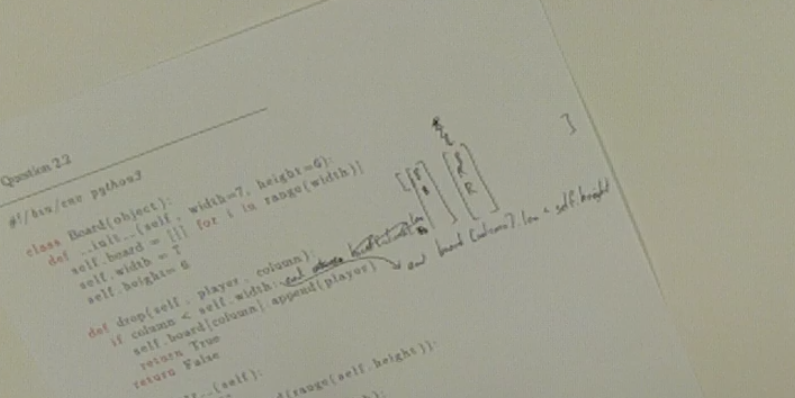
\includegraphics[width=1.0\textwidth]{2_2drawing.png}
\caption{Drawing student created during transcript line T6 and the solution he later wrote}
\label{fig-q4-drawing}
\end{figure*}

After the end of this transcript, the student identified the drop function as a point where the bug could be fixed, and did not go through any other code in the file. 
He was confident that he understood the solution to the problem even though he had only looked at a small portion of the provided code. 



%\subsection{Play-by-Play}
%\subsubsection{Q1}
%\begin{tabular}{lp{13cm}}
%1& Alright so, its got a main, so that gonna start. [...]\\
%\end{tabular}\\
%The student is going to start with the main function, which gets called at the bottom of the script. \\
%Omitted is the transcript of the student continuing to follow the execution until the time he reaches function 2. \\ \\
%\begin{tabular}{lp{13cm}}
%2& Function 2 returns function 1 with the same two arguments already passed to it,\\
%3&and function 4, the result of - \\
%\end{tabular}\\
%The student is evaluating function 2.
%He notes that there is function 4, and he tries to determine what the resulting value should be. \\ \\
%\begin{tabular}{lp{13cm}}
%4&Which doesn't have any implied arguments, thats interesting. Umm, \\
%5& thats, odd [pause] \\
%\end{tabular}\\
%The student is looking for implied arguments to function 4. \\ \\
%\begin{tabular}{lp{13cm}}
%6& lets see, so its calling functi-,ooh, it calling function 1.\\
%7&There we go. Uhh, yes, so its calling function with a list a number, the array and 4,\\
%8&and the function 4 as sort of a multiplier.\\
%9&A function to apply. \\
%\end{tabular}\\
%The student continues to function 1 and notices how the argument is being used.
%He then deduces the correct semantics for the function call in function 2. \\


%\newpage
\subsection{Relations Between Evaluation and Debugging}
%All line numbers in the following paragraphs refer to line numbers in the transcript of the corresponding problem. \\
%
%The student is evaluating in execution order in Q1.
%The student is unfamiliar with the semantics of passing a function as an argument in Python.
%Initially, as demonstrated on line 3 of Q1, he tries to call the function which led to confusion since there were no arguments. On line 4 of Q1, he looks for implied arguments, further evidence that he is trying to call this function.
%However, by continuing in execution order to function 1,he is able to notice how the argument he had tried to call earlier is now being used as a function to apply, as stated in line 9 of Q1.  \\
%
%The student is debugging by reading from top down, stopping upon encountering a likely solution, in Q4.
%Upon reaching the creation of the board data member, the student's lack of experience with Python causes him to be confused about how the physical representation of a connect four board maps onto this data member.
%As he continues reading top down, the Python list functions used in the drop function help him determine which of the possibilities (previously enumerated on line 3 of Q4) were true for the board data member.
%This helped him map the physical representation onto the data member.
%This knowledge helps him fix the bug which had been given to him in relation to the physical connect four board.  \\

The student used two different strategies in the debugging and evaluation question which helped him move past an unfamiliar concept each time. Despite using different strategies, each strategy was clearly an efficient method to solve each problem. For example, in other interviews, if the student did not move directly from function 2 to function 1 in Question 1, it took much longer to connect function 4 from being passed as an argument to being an applied function in function 1. In Question 4, some other strategies we have seen have led the student to get stuck in other locations as they tried to relate the code to the physical model. Thus, being able to solve a problem efficiently requires the student to choose an effective strategy. 





%The right method can help a student move past concepts they are not familiar with. While evaluating, a student used execution order which helped him understand a concept, and switching to top down let him ignore a large portion of the code and clear up some misunderstandings.


\subsection{Summary}
We have shown that a student used different strategies to decide which order to look at functions within two problems, and that each chosen strategy appeared to help him understand an unfamiliar concept.
For the evaluation problem, the student evaluated the code in the order it would have been executed. 
In the process, he was initially confused by the code passing a function as an argument, but realized what was happening by continuing to follow the path of execution. 
For the debugging problem, the student started looking at the code at the top of the paper and continued down until reaching a likely candidate for the location of the bug. 
As he debugged, he was initially unsure about the data structure used as the board data member, but as he continued down, he was able to find code that supported one of the possibilities he had enumerated earlier.
For this student, each strategy appeared to help him understand unfamiliar constructs, allowing him to solve the problems. 

%\newpage
